% $Id: design.tex 269 2003-04-22 14:45:04Z mackers $
\section{Requirements}

This chapter will outline the requirements of the table repair tool from
a user, domain and system point-of-view.

\subsection{User Requirements}

\label{userreqs}

\subsubsection{Importing Documents}

\strong{The user will be able to import documents using a standard open dialog
box.} The application supports any document authored in Word 97, Word 2000,
Word XP, Excel 2000, Excel XP, FrontPage or Dreamweaver. Documents saved in
future versions of these applications as well as any reasonably well-formed
generic HTML should also be anticipated and supported. The application may be
later extended using external import filters to support other formats such as
CSV or RDF. The CSV filter will be implemented as an example of how to do this.

Upon selecting the document to import, the application will display the
table(s) in that document, ready for editing or exporting. Only one document
may be opened simultaneously.

\subsubsection{Document Content}

\strong{Document content outside of tables will not appear in the application
window, but will be preserved in the output document. Furthermore, this content
will be converted to valid XHTML 1.0 Strict.} This may mean some structure may
be altered to become more structured and/or accessible, however no content will
be lost in the conversion. Exported XHTML documents will be \emph{cleaned} to
remove font tags and change presentational tags to logical tags. Other (non
XHTML) output formats may discard non-table content.

\strong{Styles and formatting in the table itself will not appear in the
application window.} This is to reduce visual congestion and to emphasise the
table headers when displaying the table (these are displayed in bold). The
structure (i.e. HTML markup) of individual cells may change in the conversion
process in order to conform to the XHTML 1.0 Strict standard or to maintain the
same level of accessibility across the table. For example, bold tags will be
changed to strong tags. However, fully accessible HTML for non-table elements
is outside the scope of this application. If possible, the user should avoid
including non-table elements (e.g. images, fonts and embedded objects) in the
input documents.

\subsubsection{Table Structure Preservation}

\strong{The existing table structure and attributes will be preserved during
the importation process.} The imported table(s) will have the same number of
rows and columns as the original document. The table's summary, caption and
other attributes will be preserved.

\subsubsection{Table Header Identification}

\strong{The document parser will make a reasonable attempt to identify the
headers and sub-headers for each table and display the headers for the user to
verify or adjust.} This will be achieved using any existing header markup in
the original document. If no existing markup exists, the parser will attempt to
identify headers by examining other markup and styles. No distinction is made
between headers and sub-headers.

\subsubsection{Table Navigation}

\strong{The application supports multiple tables in the document, and will
provide a mechanism for switching between tables.} A maximum of ten tables is
supported. Nested tables (i.e. a table inside another table) and tables for
layout purposes are not supported. Documents containing either of these types
of table will not be imported.

\subsubsection{Specifying Table Information}

\strong{For each table in the document, the user shall be able to specify the
table summary and caption.} This functionality will be provided using text
input boxes in separate dialogs. The application will \emph{not} provide
default values for these required data fields in order to encourage the user to
enter these values. The application will not export a document containing
tables that have no summary or caption information.

\subsubsection{Cell Highlighting}

\strong{Multiple cells may be selected in order to perform an operation on more
than one cell}. By using the shift key or other modifier, it will be possible
to highlight or select multiple cells. Certain operations can then be performed
on this group of cells.

\subsubsection{Header Associations}

\strong{It will be possible to manually edit the header associations for each
cell or group of cells using a separate dialog box.} This will allow expert
control over each cell, by giving the user access to the internal hierarchal
structure of each table. This is achieved by referencing associated header(s),
using their unique identifiers. This text box is accessed via a menu item and
is available for both normal cells and for headers cells (which may in turn
have super-headers). Cells may have associations with one header or with many
headers or sub-headers on preceding rows or columns. 

\subsubsection{Header Information}

\strong{It will be possible to edit the abbreviation, ID and axis for any
header.} This information can be edited via separate dialog boxes accessed
from a menu. Abbreviations will be limited to 10 characters and may not exceed
the length of the header label. Header IDs are automatically assigned. Cell
axes are optional.

\subsubsection{Status Bar}

\strong{Information on the currently highlighted cell(s) is displayed in a
status bar.} For normal cells, the header associations and the cell axis (if
any) is displayed. For headers, the ID and the header abbreviation will also be
displayed.

\subsubsection{View Source}

\strong{The current document source will be available via a menu item}. The
source will be displayed in a separate window and will reflect the state of the
document's tables at that moment in time. The source will be in XHTML
regardless of what export format the user ultimately chooses.

\subsubsection{Exporting Documents}

\strong{When the user judges the structure of the table(s) is satisfactory, the
user shall export the document using a standard `Save As' dialog}. The default
output format is XHTML 1.0 Strict. 

Other output formats may be implemented at a later stage and will be included
in this dialog. Examples of other output formats are CALS\footnote{CALS is the
table structure used by the DOCBOOK format} and HTML 4.0.

The application will be able to re-import exported documents, however it is not
required that the application retain the header association information that
has been saved, and so these documents will be treated like generic XHTML.

%\subsubsection{Command Line Scripting}

%\strong{It will be possible to autonomously and automatically instruct the
%program to perform conversions from the command line.} This will be only
%possible with documents containing one table and requires that some
%information be passed to the program as command line arguments, such as the
%table summary and caption. The quality of this result will vary depending on
%the input document and the program's ability to identify headers in the
%document. So, while results may not be as accurate as the interactive method,
%the program may be interfaced with other applications or on websites.

\subsection{Domain Requirements}

\subsubsection{XHTML 1.0 Strict Compliance}

The primary output format is HTML. The HTML is intended to be as accessible as
possible. Rather than choosing a pure HTML standard, such as HTML 3.2 or HTML
4.0, the program will use the XHTML~\cite{w3c:xhtml} output format. 

\begin{quotation}

The Extensible Hypertext Markup Language (XHTML) is a family of current and
future document types and modules that reproduce, subset, and extend HTML,
reformulated in XML. XHTML Family document types are all XML-based, and
ultimately are designed to work in conjunction with XML-based user agents.
XHTML is the successor of HTML, and a series of specifications has been
developed for XHTML.

\end{quotation}

XHTML has a number of benefits over standard HTML:

\begin{itemize}

\item XHTML documents are XML conforming. This means that they can be edited,
viewed and validated with existing XML applications.

\item XHTML documents can seamlessly be viewed and parsed by existing HTML
tools and browsers.

\item XHTML documents can be parsed using the document object model, allowing
for automated scripts or agents better access to the content of the document.

\item XHTML is rapidly being accepted as the replacement for HTML, with new
standards and tools being development to take advantage of the format.

\end{itemize}

As XHTML can be parsed by existing and older browsers, the end user should not
be concerned that the document is actually XHTML. Instead it makes sense to use
this newer standard in order to avoid future deprecation. What's more, because
the DOM is extensively used to manipulate the source documents, XHTML is
explicity implied, which simplifies the generation of the output document.

\subsubsection{W3C Web Content Accessibility Guidelines 1.0}

The W3C Web Content Accessibility Guidelines~\cite{w3c:wcag} (also known as the
Web Accessibility Initiative (WAI) Guidelines) explain how to make web content
accessible to people with disabilities. They are intended to advise page
authors, site designers and developers of authoring tools on how to make web
content more available to all users, whatever user agent they are using or
constraints they may be under. 

The output document will conform to Guideline 5, which is ``Create tables that
transform gracefully''. It is advised to ``ensure that tables have necessary
markup to be transformed by accessible browsers and other user agents.''

As a secondary objective, a reasonable attempt will be made to ensure
that the rest of the document conforms to some of the other guidelines in this
document, specifically those that can be automated, as no data will be obtained from
the user on these elements.

This document will also extensively make use of W3C's document on Techniques
for Web Content Accessibility Guidelines~\cite{w3c:wcagtechs}, which includes
methods and techniques for satisfying the requirements defined in ``Web Content
Accessibility Guidelines 1.0''.

\subsubsection{Section 508 Compliance}

In 1998, the United States Congress amended the Rehabilitation Act to require
their electronic and information technology accessible to people with
disabilities. Section 508~\cite{section508} is the manifestation of this
amendment.

The output document will conform to part 1194.22 of this document governing
``Web-based intranet and Internet information and applications''.

\subsubsection{Irish Government Website Accessibility Regulations Compliance}

The Irish Government's Public Service Web Standards states that Irish public
service web sites must conform to the WAI Guidelines and the Irish Public
Service Meta-data Standards~\cite{irishgov}.

While it has been established that the document will conform to WAI Guidelines, it
will also be ensured that the meta-data standards are maintained.

\subsubsection{W3C Authoring Tool Accessibility Guidelines} 

The W3C also provides guidelines for developers creating \emph{authoring
tools}\cite{w3c:atag}. The program will adhere to these guidelines.

By its very nature the program will support accessible authoring practices
which will be part of its look and feel. The produced output will be valid
XHTML and have no non-accessible content. The program will not output a file
that contains non-accessible tables, and will prompt the user in this case.
Additionally, each dialog box will document whatever feature it pertains to.

The program itself must also be accessible to people with disabilities. To do
this, it will make full use of the Java Accessibility Utilities, which are a
set of utility classes that help assistive technologies provide access to GUI
toolkits that implement the Java Accessibility API.

%\todo{More details on Java Accessibility API.}

\subsection{System Requirements}

\label{sysreqs}

\subsubsection{Window Appearance}

The main application window is not unusual in that it consists of a title bar, a
menu bar, a status bar and a content pane. When the application is first
loaded, the content pane and status bar will be blank, and the title bar will
have an enabled `File' menu and a  disabled `Table' and `Cell' menu. The `File'
menu will have enabled `Import' and `Exit' menu items and disabled `Export' and
`View Source' menu items.

Importing a document will cause the `Export' and `View Source' menu items and
`Table' and `Cell' menus to become enabled. The state of the menu items of the
latter two menus depends on what cells are selected. It is not possible to
close a document once it has been opened, but another document may be imported.

The look and feel of the application will use Swing's system dependant look and
feel. For example, when running the application on Microsoft Windows, the
application will use Windows' native widgets, icons and cursors.

Each user interface string will be read from a separate Java properties file.
This will allow easy localisation of the application into other languages.
A French version of the program will be provided as an example of how to
localise.

\subsubsection{Importing Documents}

The import feature is accessed via an `Import' menu item in the `File' menu.
Selecting this item will open up a standard `File Open' dialog box from which
the user may select a document. The default filter is `HTML Files' which
includes all files with `htm' in their extension, e.g. .htm, .html, .xhtml,
.HTML. Other filters included are `CSV files (*.csv)', `RDF files (*.rdf)' and
`All Files'. 

If a document is already open that has not yet been exported then a
dialog will ask the user if the open document should be exported first.

Each supported document type has its own \emph{Importer}, which knows how to
handle that document format. Each importer is an implementation of a common
interface, and so share the same methods and return types. The importers are
given the inputstream connected to the document that is being imported and are
expected to return a document object, which can then be handled uniformly by
the remainder of the import process.

The type of importer to use is determined by the document's extension. The file
extension is the part of the filename after the last period. For example, in
`index.html', the extension is `html'. Each supported importer and its
associated extension and import techniques is described below. Files with no
extension or an unrecognised extension are assumed to be HTML and thus use the
HTML Importer. File extensions are listed and match in both upper- and
lower-case forms, or a combination of the two.

The import process may take a short while to complete. In order to inform the
user that something is happening, the mouse cursor changes to its `wait' state
for the duration.

\subsubsection{The CSV Importer}

The CSV (Comma Separated Values) file format is a plain text file consisting of
multiple lines of data. Each line consists of a number of fields of data
separated by commas. Each field may be enclosed by double quotation marks. CSV
lacks any mechanism for distinguishing between header and content data, so is is
assumed that all the data is content. The CSV format is a supported output
format of a number of applications, such as Microsoft Excel and various
database systems, and so it would be desirable to support this import format.

The CSV Importer is implemented as a subclass of the XHTML Importer (see
below). This may seem strange, but in practise it is useful to use the XHTML
Importer's routines after the CSV has been converted to XHTML. This is done using
Doug Tidwell's CSV to HTML
converter\footnote{http://www-106.ibm.com/developerworks/xml/library/x-xmlexperts-csv/}.

The CSV Importer is used for any document with the `.csv' extension.

\subsubsection{The RDF Importer}

RDF (The Rich Text Format) is a standard document format used for distributing
documents among workgroups where Microsoft Word or any other proprietary
document format is not universally supported. RDF can be outputted from
Microsoft Word and other popular word processing software.

The RDF Importer will not be implemented at this stage, but hooks in the code
will allow the class file to be implemented and inserted at some later time. If
the filter is not found, then an exception will be thrown and an appropriate
error message will be displayed.

\subsubsection{DOC and XLS Documents}

The program will not support Microsoft Word's or Microsoft Excel's native
proprietary format (with `.doc' and `.xsl' extensions respectively). Any
attempted by the user to load one of these document will result in the display
of an error message inform the user that the program cannot read these file
formats and to use Word's or Excel's \emph{Save As HTML} feature.

\subsubsection{The XHTML Importer}

Documents with an `.xhtml' extension are opened using the XHTML Importer.
Because XHTML is a XML format, Java's XML parser can be used to open the
document, which will construct a document object from the file. If the XHTML
file is not well-formed, then an exception will be thrown and an error message
will be shown. XHTML documents with a different extension will be handled by
the HTML importer (see below), which will ultimately return a copy of the
original document.

\subsubsection{The HTML Importer}

Other files with an extension containing the string `htm' (e.g. `.htm',
`.html', `.shtml' and `.HTML') as well as files with unknown or missing
extensions are opened with the HTML Importer. The HTML Importer parser then
uses the following steps to create the document object.

\begin{enumerate}

\item Because this filter is the default filter, it must be verified that the file
is in fact HTML. To do this, the file is searched for an opening tag.  Any
particular opening tag cannot be searched for ( for example, `head' or `body')
as the HTML file may only be a fragment of another complete HTML file. This may
occur, for example, if the user copies out a table and pastes into a new file. 

Instead any opening tag is searched for, in the form of a less than sign ($<$)
followed by one or more alphanumeric characters and a space or greater than
sign ($>$). If one of these is found, it is assumed that the file is HTML. Of
course, this may occur coincidently in another non-HTML file. 

If the file does not appear to be HTML, and exception will be thrown and an
error message is displayed.

\item Next, the type of HTML document is determined. This is in order to run the
document through the correct \emph{preparser} (see below). It may be accurately
determined in which program the document was authored in (if any) by looking at
the `generator' meta tag. For example, documents authored and saved as HTML in
Word 97 have the meta tag\\ \code{<META\ NAME=``Generator''\ CONTENT=``Microsoft\
Word\ 97''>}\\. Now that is has been determined that this document was created in
Word 97, the preparser can be given clues on how to treat this file.

The exact format of the generator tag may vary slightly, e.g. use of double or
single or no quotes in either the name or content or both attributes, or and
upper- or lower-case `generator' attribute. A \emph{regular
expression}\footnote{Regular expressions are a standard way to search for
patterns in text strings, and are implemented in Java version 1.4 and later.}
will be used on the whole document string to pull out the generator tag.

Although unlikely, if may be possible that the document was saved in a version
of Word, and edited later by hand. This would leave the generator tag, but the
HTML source may not match what was expected from the Word version. In this
case, the robustness of the HTML parser will handle this to a certain extent
without a preparser.

\begin{table}
\begin{center}
\begin{tabular}{ll}
\strong{Product Version} & \strong{Generator Tag} \\
Microsoft Word 97 & Microsoft Word 97  \\ 
Microsoft Word 2000 & Microsoft Word 9 \\ 
Microsoft Word XP & Microsoft Word 10 \\ 
Macintosh Word 98 & Microsoft Word 97/98 \\
%Macintosh Word 2000 & \todo{word2kmac Generator Tag} \\ 
%Macintosh Word XP & \todo{wordxpmac Generator Tag} \\ 
Microsoft Excel 97 & Microsoft Excel 97 \\
Microsoft Excel 2000 & Microsoft Excel 9 \\
Microsoft Excel XP & Microsoft Excel 10 \\
%Microsoft Frontpage & \todo{frontpage tag} \\
%DreamWeaver & \todo{Dreamweaver tag} \\
\end{tabular}
\end{center}
\caption{Generator tags written by different programs}
\label{table:generators}
\end{table}

The type and version of HTML may also be determined using the document's
\emph{DOCTYPE}, if present. The DOCTYPE is a special tag that may or may not
occur in HTML files and will always occur in XHTML files. Using the DOCTYPE it 
can be determined if the file is HTML or XHTML and what version of that format. An
example of a DOCTYPE is $<$!DOCTYPE\ HTML\ PUBLIC\ ``-//W3C//DTD\ HTML\
4.0\ Transitional//EN''$>$. From this it is known that the document is HTML 
version 4.0 Transitional. As all the supported programs correctly output a
generator meta tag, DOCTYPE checking does not need to be implemented.

\item If the previous step identified a supported generator, then the document
can be run through a relevant preparser. Each supported program will have a
corresponding preparser. 

The purpose of pre-parsing is to ensure that successive stages can successfully
read the HTML document. Any bugs, inconsistencies or malformed source found in
the HTML source can be removed or repaired at this stage. Extensive testing
will reveal malformed input HTML generated by Word, etc. It may be the case
that many pre-parsers are not needed.

Regular expressions will be used to search for problematic markup in the
document and replace with something the HTML parser can deal with.

If no supported generator tag was found (i.e. the document is generic HTML),
then the document is run through a \emph{null preparser} which does not perform
any pre-parsing on the document and returns it unchanged. This is because it may
be impossible to compensate for the sheer number of combinations of generic
HTML which may be written by hand or generated by an unsupported document type.
Instead it is trusted that the robustness of the HTML parser (see below) can handle
these documents.

\item The next stage is to run the input document through a program called
\emph{Tidy}. Tidy is a program used to `clean up' HTML, as well as perform
other functions such as removing unwanted and unnecessary tags and converting
presentation tags to logical tags (e.g. `b' to `strong'). Tidy is by no means
perfect, as it may sometimes reject certain HTML documents. However, most of
this problem HTML should have been eliminated in the previous pre-parsing stage.
The program will use an Java implementation of Tidy call \emph{JTidy}. 
%The exact operation of JTidy can be controlled by the user and is discussed in full in Appendix \todo{JTidy appendix}. 
If JTidy fails to parse the document, then an exception will be thrown and the 
user will be advised to manually repair the document and to try again.

JTidy will be used to convert the HTML document into XHTML (version 1.0
Strict). Because XHTML is valid, well-formed XML, the document can be parsed as
XML and a document object can be created, which can be used in the next stage in the
import process. 

The HTML Importer will be imported as a subclass of the XHTML importer. This is
so that, once HTML is converted to XHTML, the XHTML can be reused in the 
Importer's routines for accessing the structure of the document.

\end{enumerate}

\subsubsection{Table Checks}

The previous stage has ensured that, whatever the original document type was,
the document is now in a form that can be used uniformly. This form is as a
document object, which is part of the the DOM\footnote{The Document Object
Model API allows programmers to access any part of an XML document in a
hierarchical manner. For more information see http://www.w3.org/DOM/} API. 
This API is used to dynamically access the content and structure of the document in
a hierarchical manner, allowing us to isolate each table element and operate on
its contents independently. The \code{org.w3m.dom} package provides the Java
interface to the DOM. This package is free to use, and its API well documented.

The DOM is first used to perform the following checks on the document. If any of
these checks fail, then an exception will be thrown and a suitable error
message will be displayed to the user.

\begin{itemize}

\item The document must contain at least one, and not more than ten tables.

\item The document must not contain any nested tables. A nested table is a
table contained inside another table, and is tested for by checking each table
element for a DOM descendant which is also a table element.  Nested tables are
not supported because it is not recommended by WAI guidelines.

The document must not contain any layout tables. A layout table is considered to
be a table where one cell contains more than quadruple the amount of text of
the next most populated cell. Layout tables are not supported because WAI
guidelines do not recommend using header markup for them.

\end{itemize}

\subsubsection{Table DOM Parsing}

Although the DOM structure of the document is useful, it is advantageous to convert
each table into an internal data structure. This has its advantages both for
speed and for ease-of-use. Each table and each cell will need its own object to
store additional attributes and to perform routines on.

To this end, the DOM structure of each table must be traversed to construct a
two-dimensional array of cells to represent the real table structure. This
array has a size of rows by columns. The number of rows in a table is equal to
the count of the TR elements in a table. The number of columns in a table is
determined by either

\begin{itemize}

\item summing all COL elements (including those with a `span' attribute), all
empty COLGROUP elements with spanning and all COLS in each non-empty
COLGROUP element (ignoring `span' attributes),

\item or taking the row with the highest number of cells (including header
cells and spanning cells).

\end{itemize}

Once the array has been created, the table is iterated through row by row and
cell by cell, creating a cell object in the array for each DOM cell element. 
The following caveats of table structure must be dealt with to ensure 
the array is created successfully:

\begin{enumerate}

\item Rows which contain more cells than the COL or COLGROUP elements allow
will have the trailing cells dropped.

\item Rows may contain less cells than the COL or COLGROUP elements specify.

\item Row and column spanning must also be supported. This is achieved by
inserting \emph{Null Cell} objects into spaces where cells span. For example,
if a cell spans for three columns (i.e. its HTML attribute is
\code{colspan="3"}), then the two cells immediately below this cell become null
cells. When inserting cells in the next two rows of the table, the algorithm
will skip these null cells and fill the cell to the right instead. Similar
behaviour is implemented for cells that span rows and cells that span both rows
and columns.

\end{enumerate}

\subsubsection{Table Headers Identification}

At this point, the program will attempt to identify the natural, logical
headers for each table, using one of the methods below. Each header cell
identified becomes a special \emph{Header Cell} subclass of the generic cell
class.

\begin{enumerate}

\item If the table contains `th' elements then it is assumed that the logical
structure of the table has been preserved. These elements will be used to
determine the location of the table headers without searching for any other
table headers.

\item If no header elements are found, but there is a `thead' element, then 
all cells inside this element are turned into header cells.

\item If the above methods fail, it is assumed the logical structure of the
table has been lost, and style or formatting patterns in the table must be
looked for in order to determine which cells are headers and which are not. It
is not sufficient to simply label the first row and/or column as a header, as
the table may also contain sub-headers. A header can be defined as a cell in
which the entire textual content is enclosed in a bold tag (actually a strong
tag after tidy processing). If any text is outside such a tag, then the cell
does not qualify.

\end{enumerate}

At this stage, any table header without a header ID attribute (maybe from the
original HTML document), will be assigned one. The assigned identifier will be
unique across the whole document\footnote{The `id' attribute must be unique
across the whole document to prevent id clashes with other (possible non-table)
elements.}, and will take the form of the letter `h' followed by a number which
is incremented for each new header. When an ID is assigned, it will be checked for
its uniqueness across the document and continue to increment the number until a
suitable unique id is found.

\subsubsection{Header Association Identification}

If table headers are found, then the program will attempt to find what cells
are associated with these headers, using the following methods:

\begin{enumerate}

\item If a cell has a `headers' attribute, then each header listed in the
attribute will be associated with that cell.

\item If a `scope' attribute appears in a table header, then the program will
associate all cells within the range of that scope with this header. Table
headers with a `row' scope will cause all cells on the remainder of that row to
be associated with that header. Similarly with a `col' scope, all cells below
that header are associated with it. The program does not support `rowgroup' or
`colgroup' scopes.

\item For any cell which still does not have any header associations, 
the following algorithm will be used to find an associated header:

\begin{enumerate}

\item Search left from the cell's positions and record table headers, then
search up from the cell's position and record table header cells. The search in
a given direction stops when the edge of the table is reached or when a data
cell is found after a header cell.

\item Row headers are inserted in the list from left to right. Column headers
are inserted into the list from top to bottom.

\item If a header is found that has a `headers' attribute set, then the headers
referenced by this attribute are added to the list and the search stops for the
current direction.

\end{enumerate}

\end{enumerate}

\subsubsection{Table Display}

If more than one table exists in the document then the first consecutive table
in the document will be displayed first. 

Any styles or formatting in the table will not be displayed. This is to reduce
visual congestion and to emphasise the table headers when displaying the table.
Table headers are displayed in a bold font, with regular cells displayed in
normal font. The cell background colour is white and text colour is black,
unless the cell is highlighted, in which case the background colour is blue. Light grey grid lines are displayed between cells. 

Null cells (i.e. cells that have been spanned) are displayed blank with a grey
diagonal line through them. They cannot be highlighted. The content of the
spanning cell will appear in the first cell position only.

%Each column and row of the (visual) table starts with a small button. Clicking
%the button will highlight that entire row or column. This is a similar
%behaviour to that seen in spreadsheet programs such as Microsoft Excel.

A customised version of Swing's\footnote{Swing is a graphical toolkit for Java,
which will be used exclusively for the GUI in this application} JTable class
will be used to display each table in the document. JTable allows us to include
styled text for the data and paint lines for null cells.

Each table will be placed in a scroll-able pane which will display a vertical
scroll bar for long tables. Horizontal scrolling will not be available.

Column groups will not be rendered in any fashion.

The textual content of the cell may be visually truncated or shortened to
display correctly in a table cell. No formatting, images or other elements will
appear in the table, except to distinguish table headers.

The table `dir' attribute is not supported, meaning that only left-to-right
direction tables are supported.

\subsubsection{Table Navigation}

If a document contains more than one table, then other tables may be accessed
via the `Tables' menu. The Table menu gives a list of tables in the document
using the tables' captions (or `Table 1', `Table 2', etc. if not defined). In
order to ensure the menu doesn't exceed the screen width, only the first
12 letters of the caption will be displayed and a maximum of 10 tables in the
HTML document is supported.

Switching tables does not require the document to be exported, as each table's
state is maintained between switches and all tables are opened simultaneously.
Switching tables replaces the content pane of the window with the selected
table's scroll pane.

\subsubsection{The Title-bar}

The window's title consists of the name of the application followed by the
document's title (or its filename if not defined) followed by the table's
caption (or the table number if not defined).

There is no limit on the length of the title, as this will be handled by the
window manager.

\subsubsection{Status Bar}

If a header cell is selected, the status bar will display the header ID and the
header abbreviation. Highlighting multiple headers will clear these values.

If a cell has any header associations, then these will also be displayed in the
status bar. This takes the form of a comma separated list of header cells
(using their abbreviation, content or id). Highlighting multiple cells will
cause the status bar to show the associations for all cells, but only if their
associations are identical.

If an axis is present for a cell, this will be also be displayed. Selecting
multiple cells will clear the axis status, unless the selected cells share a
common axis.

To ensure visual consistency, each field in the status bar (id, abbreviation,
associations, axis) will appear in a different `cell' of the status bar. The
id, abbreviation and axis cell will remain at a constant size. The associations
cell will resize when the window is resized.

\subsubsection{Highlighting Cells, Rows and Columns}

Individual cells are selected or highlighted by clicking on the cell. If the
cell is not already highlighted, then it will become highlighted. A second
click on the cell will un-highlight it. Unmodified clicks to a cell will cause
all other cells to be un-highlighted.

If another cell is clicked with the `shift' key depressed, then all cells
between this cell and the currently highlighted cell will become highlighted.
This behaviour is intuitive and common in table-based applications.

More cells can be added to the range of highlighted cells by shift-clicking
further cells. Ranges of cells must be continuous.

\subsubsection{Specifying Table Information}

The currently selected table's caption and summary can be edited by selecting
`Edit Caption' and `Edit Summary' from the Table menu respectively. The caption
will be editable via a single line text box, and the summary via a multi-line
text box.

The W3C guidelines~\cite{w3c:wcagtechs} state the caption should be one to
three sentences in length. An estimation of an average sentence size is around
80 characters long, so the caption will be limited to 240 characters in total.

There are no explicit restraints on the table summary in any accessibility
standards, however it would be desirable to limit the size on this to a reasonable
length, say 2000 characters.

These dialog boxes will have a description of the purpose of the table summary
and caption.

\subsubsection{Specifying Header Information}

Header information for the currently selected header cell may be updated using
the `Edit Header Info' menu item of the `Cell' menu. The unique header
identifier and the header abbreviation (if any) will be displayed. The user may
edit both values. 

The ID must be unique across the document, contain no non-alphanumeric
characters and be no longer than 10 characters. Changing this value will update
all references to this header.

When the dialog is closed, the program will check that this header is unique,
that the abbreviation is not longer than the actual header cell value and that
the abbreviation is not longer than 10 characters.

This menu item will be unavailable if a non-header cell is selected, or if more
than one cell is selected.

This dialog box will have a description of the purpose of the header ID and
abbreviation.

\subsubsection{Specifying Cell Axes}

The `axis' of a data or header cell can be specified using the `Edit Axis'
menu item of the `Cell' menu. The axis of a cell is a free-form string to add
semantic meaning to a data or header cell.

The axis is an optional attribute and is not required to output an accessible
document, and is not used by any mainstream browsers. However it is useful to
allow users to specify this attribute to `future-proof' the document, if future
browsers or data analysis tools where to make use of this.

Multiple axes may be specified by separating the string with commas.

Some constraints will be enforced on the axis string. Firstly, the string may not be
longer than 20 characters per comma. Secondly, the string may not contain a
space or any punctuation characters (other than a comma). This is ample freedom
to pick a suitable string, but should ensure compatibility with future user
agents.

This menu item is available if multiple header or data cells are selected and
the dialog will contain a description of the axis attribute.

\subsubsection{Adding and Clearing Headers}

Headers may be associated with cells by using the `Add Header' menu item of the
`Cell' menu. This will present the user with a drop-down list of current table
headers (using their abbreviation, content or ID). The dialog will have a
description of what headers associations are used for.

The user chooses a header, clicks `OK' and the chosen header is associated with
the currently selected cell(s). The current header associations are not
affected. A maximum of 10 headers can be associated with a cell and an error
message is displayed if the header list is full.

The user may clear the list of associated headers by selecting the `Clear
Headers' menu item of the `Cell' menu. This dialog-box-less menu item has the
function of clearing the list of associated headers for the currently selected
cell(s), this allowing the user to add up to ten more headers.

A third menu item labelled `Add Header Scope' is available when one or more
header cells is selected. Two options are given by this dialog box, `Row' and
'Column'. Selecting either of these has the effect of associating all cells to
the right of this header with it (row), or all cells below it with it (column).
This dialog has a description of what header scope is.

These menu items are not available if no cells are selected.

\subsubsection{Changing Cell Types}

Content cells may be changed to header cells using the `Make Header' menu item
of the `Cell' menu. This has the effect of changing the program's internal
representation of the cell to be a header cell. A unique ID will be given to
the cell.

Conversely, a header cell may be changed into a content cell using the `Make
Data' menu item. The header ID and abbreviation is discarded and all cells
associated with this cell will have the header dropped from the list of
headers.

\subsubsection{Viewing Source}

At any stage it is possible to view the current source of the document.
Regardless of what export filter the user may choose to export the document,
the view source menu always views the source in XHTML. By selecting the `View
Source' menu item of the `File' menu, a new (non-modal) window is created with
a read-only text-area containing a snapshot of the current source. The HTML
source is formatted using JTidy's pretty printer. The window is closed using
the window manager's close button. 

\subsubsection{Exporting the Document}

The document is saved using the `Export' menu item in the `File' menu. This
will open a standard `Save As' dialog into which the user selects or types a
file name.

The default output format is XHTML 1.0 Strict. The document object model should
already be in this format as the import procedure converted the document to
this format and no non-valid elements were introduced. The DOM is
converted to a string and written to the location specified by the user. 
JTidy's \emph{pretty printer} will be used to output a nicely formatted document.

Before the file is saved, a number of tests are performed to ensure that the
document conforms to the desired output quality. These tests are detailed in
the `Table Accessibility' section below. If the document does not pass the
tests, the user will be informed and asked whether to preceed with the export
or not.

\subsubsection{Quitting the Program}

The program is closed by selecting `Exit' from the `File' menu. If the
currently open document has not been exported yet, then a dialog will ask the
user if the document should be exported at this stage. 

The program can also be exited using the window manager's close button.

\subsubsection{Table Accessibility}

The table HTML in the output document will conform to the following
accessibility checkpoints. If any of these checks fail when the document
is being exported, the export will abort and the user will be informed
of the problem(s) that were detected in the document.

\begin{itemize}

\item A \strong{table caption} must be provided for each table. The table
caption is provided by the user to describe the nature of the table.  The table
caption will be outputted as a CAPTION element. Although a caption is not
necessarily required, the table will not be exported if no caption is specified.

\item The \strong{table summary} must be provided by the user to provided a summary
of the relations among cells. It is especially useful for non-visual readers
and for ``tables with nested headers, cells that span multiple columns or rows,
or other relationships that may not be obvious from analysing the structure of
the table but that may be apparent in a visual rendering of the
table.''~\cite{w3c:wcagtechs}

The inclusion of a summary will be enforced for each table, and will not export
the document without. The summary is included as a `summary'  attribute of the
table.

\item Table \strong{header abbreviations} are used to cut down on repetition
and reading time when tables are read out by a screen reader, which usually
reads row and column labels for each cell. 

Header abbreviations are not required unless a table header is over 10
characters long. In this case, the program will abort the export process.
Attributes are included as a `abbr' attribute of the TH element.

\item The program will \strong{identify row and column headers} in each table using the
header information provided by the user in the previous stage. Headers are
outputted using TR tags.

%TR tags will be grouped within a THEAD and TFOOT element\footnote{the THEAD and
%TFOOT element are used to group table headers and footers and are used by some
%user agents to support scrolling of table bodies independently of the table
%head and foot} if one or more complete row of table headers is at the top or
%bottom of the table. In this case, the normal body of the table in enclosed in
%a TBODY element. Other TR elements will appear in the TBODY element. It is
%possible to have either a single THEAD or TFOOT element or both, depending on
%the position of headers in the document.

All table cells in the document must be associated with at least one header,
and the document will not be exported until all cells have been associated with
at one or more header.

%\item Wex will \strong{group columns} using COLGROUP and COL tags.

Each table cell will include a `headers' attribute to indicate the header
associations for each cell. Multiple associations will be separated by a space.
Table header cells may themselves have a headers attribute to form a hierarchy
of headers. 

The `scope' attribute of headers will not be used, as the two methods provide
the same functionality. Scope is intended to simplify manual authoring of
tables, however, as the tables are being automatically generated, it is as
simple (if not simpler) to output the headers attribute instead.

\item The axis of each table cell, if present, will be used as an `axis'
attribute of the table cell.

\end{itemize}

%\subsubsection{Scripting}

%If the program is started with a \code{-c} or \code{-s} argument, then it will
%operate in scripting mode. This mode has no graphical user interface, and will
%perform a document conversion without any input from the user. The input
%document is read from standard input and the output document is written to
%standard output. It is the responsibility of he user or script executing the
%program to handle this correctly. 

%The \code{-c} argument allows the table caption to be specified. Similarly the
%\code{-s} argument allows the table summary to be specified. For example;
%\code{-c Growth Rate -s This table shows the growth rate in the year 2002}.

%This mode should only be used on documents containing one table, as only one
%caption and summary can be expressed on the command line. 

%The program will attempt to guess the correct logical table headers in the
%usual manner.

%Tidy comes in many different flavours; from command line programs to DLL
%libraries. However, the version of tidy we will use is a Java port called
%JTidy\footnote{More information on JTidy can be found at its homepage
%http://sourceforge.net/projects/jtidy}. JTidy has a similar range of features
%to the original version (written in C). However, because JTidy is written in
%Java, it will be easier to integrate into our program while maintaining
%cross-platform compatibility.

\subsection{Non-Functional Requirements}

\subsubsection{Cross-platform}

The program will run on a large variety of operating systems and architectures,
including at least Microsoft Windows, Mac OS X, Solaris Sparc and Linux i386.
This is becoming increasingly important as non-Windows platforms are being
taken up both by developers and people with different needs. Java is inherently
cross-platform, so this requirement should not significantly increase the
amount of work needed.

\subsubsection{Modularised Code}

The code will be developed in such a manner as to maximise future code re-use
either in this project or as part of another.

The graphical user interface should be completely separate to the main
functionality of the program in so far as it is possible to implement a
text-based or web-based interface using the existing unmodified code base.

It should also be possible to implement and `plug-in' the other import and
export filters without changing the existing code.

To further assist the future improvement and development of this project by
other developers, the program should be documented using existing Javadoc
standards. This will allow an API to be created for use as a reference for
these developers.

\section{Architecture}

The architecture of the program's classes and interfaces is best described
with class diagrams. Figure \ref{fig:document-class-diagram} shows the
data structure for the document, including its tables and the different
types of cells for those tables.

Figure \ref{fig:import-class-diagram} shows the Import interface and 
implementations. It also shows the special HTMLImporter case which
requires the XHTMLConvertor and HTMLPreParser interfaces to be
implemented.

The Exporter interface currently only has one implementation, and this
is shown in figure \ref{fig:export-class-diagram}.

An outline of the graphical user interface is shown in figure
\ref{fig:gui-class-diagram}. This shows how the SWJFrame implements
the SWJTableContainer. It can be seen that the dialogs are part of
the SWJFrame while the table user interface is separated into
the SWJTable and SWJTableModel classes.

\begin{figure}
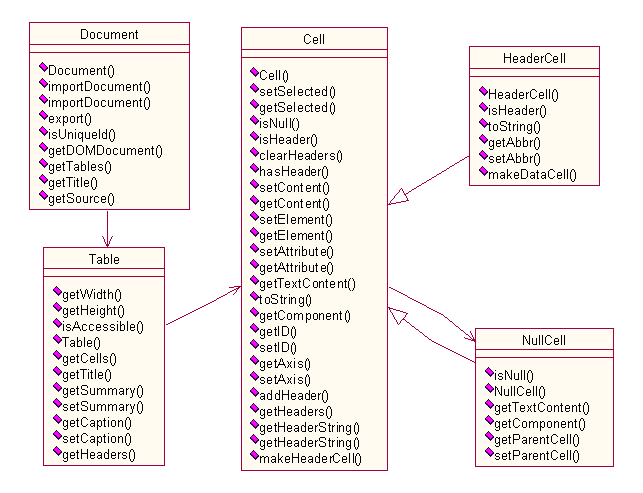
\includegraphics[width=150mm]{figures/document-class-diagram.png}
\caption{Document Class Diagram}
\label{fig:document-class-diagram}
\end{figure}

\begin{figure}
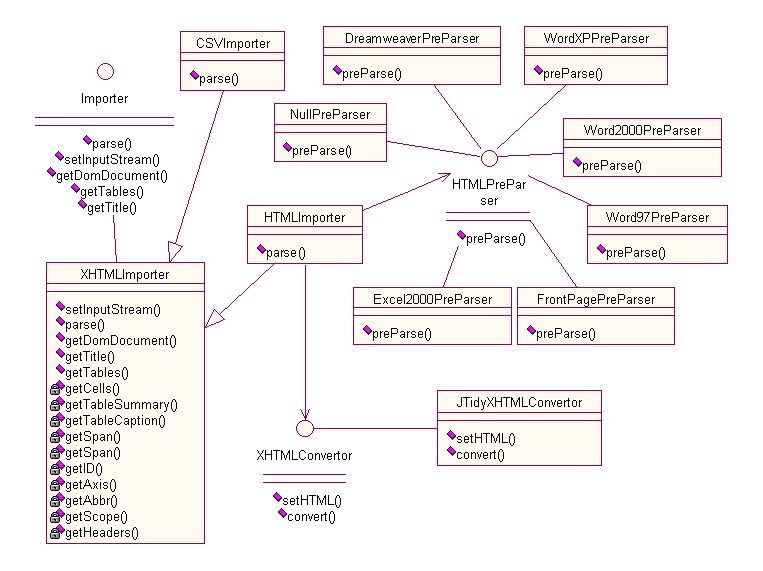
\includegraphics[width=150mm]{figures/import-class-diagram.png}
\caption{Import Class Diagram}
\label{fig:import-class-diagram}
\end{figure}

\begin{figure}
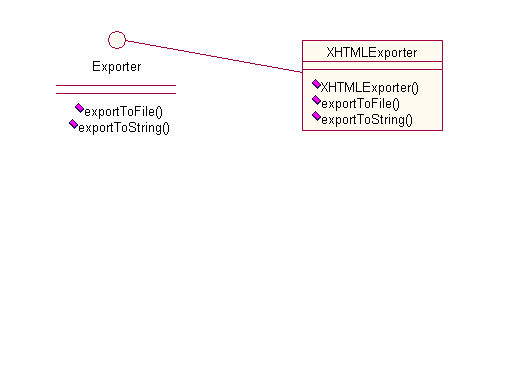
\includegraphics[width=150mm]{figures/export-class-diagram.png}
\caption{Export Class Diagram}
\label{fig:export-class-diagram}
\end{figure}

\begin{figure}
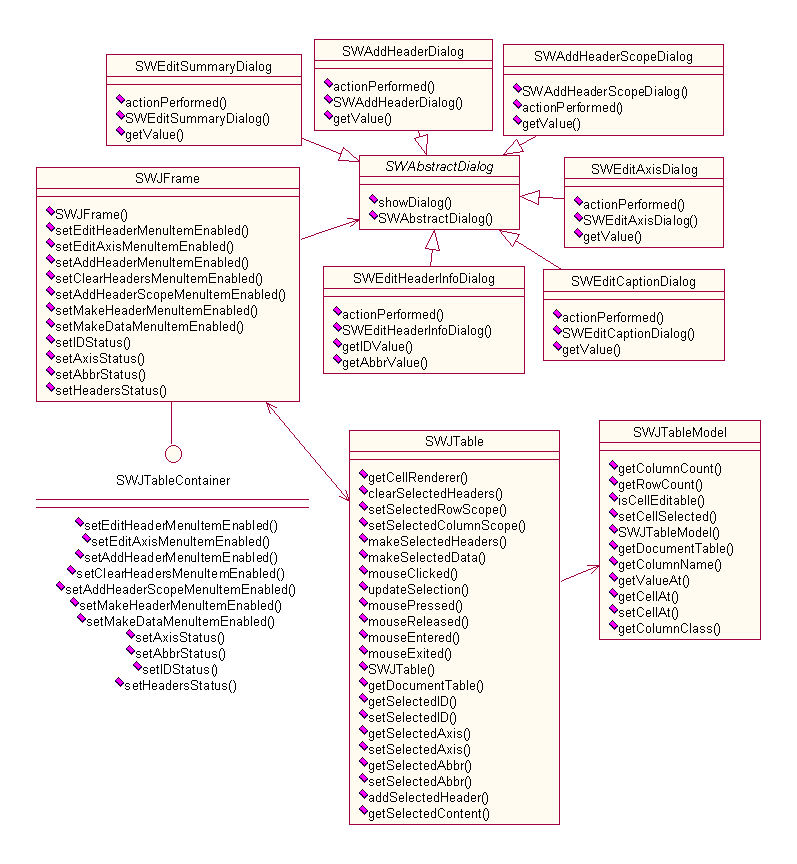
\includegraphics[width=150mm]{figures/gui-class-diagram.png}
\caption{Graphical User Interface Class Diagram}
\label{fig:gui-class-diagram}
\end{figure}

